\section{Averaged Result of Multiple Video Sequences}
\label{sec:results/section_a}

Running the experiment with all the possible combinations of QP and MSR as shown in Table \ref{tab:qp_msr_range}, we obtained the result from all the 12 video sequences or 12 samples in a statistical term. Since we have multiple video samples, we averaged each score of performance metric with respect to QP and MSR. As there are 20 metrics for evaluating object tracking performance, and MOTA is a good indicator for the general tracking performance as explained in Chapter \ref{sec:background/section_d}, we visualized MOTA score at different QP and MSR as shown in Figure \ref{fig:averaged_result_all_qp}.
\begin{figure}[!htbp]
  \centering
  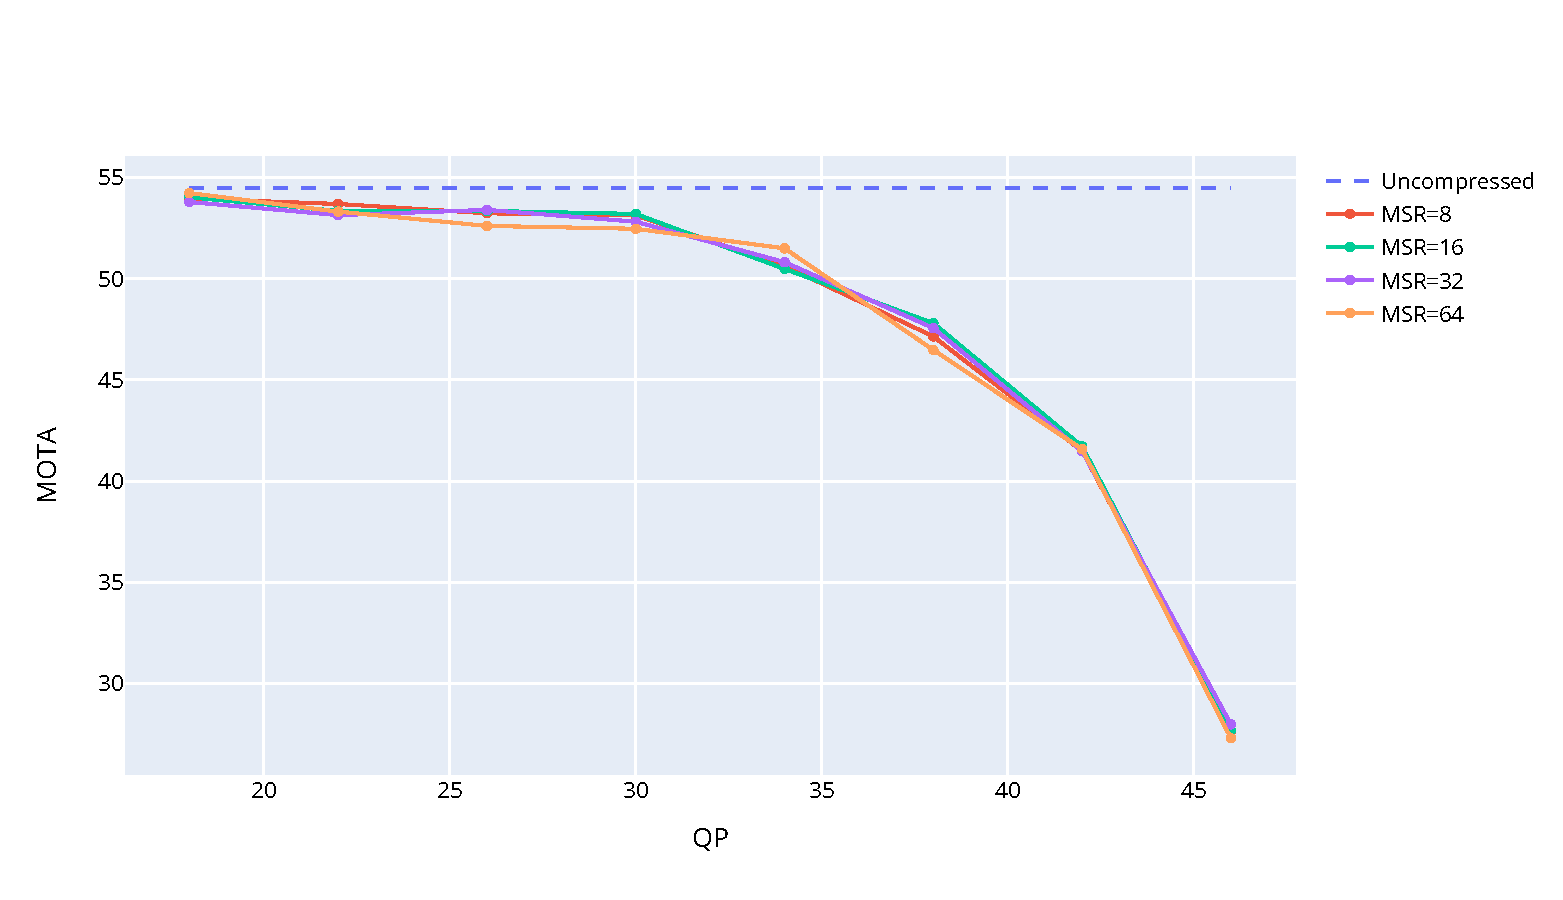
\includegraphics[width=1.0\linewidth]{img/averaged_result_all_qp.pdf}
  \caption[Averaged Result of All Video Samples with All Object Classes]{
    
  }
  \label{fig:averaged_result_all_qp}
\end{figure}
As can be seen from the plot, the uncompressed video sequences achieved the highest performance of the MOTA score. For the compressed sequences, the MOTA score is lower than the uncompressed result, and the higher the QP, the lower the MOTA score. Although the measurements at different MSR are plotted, we do not see any significant differences from this plot. Not only MOTA, we observed that the performance scores of most of the metrics decrease as QP increases. Figure \ref{fig:averaged_result_all_multiplots_qp} shows the visualization of all the metrics over different QP and MSR, and Table \ref{tab:averaged_result_all} shows the means of 12 numerical measured values.
\begin{figure}[!htbp]
  \centering
  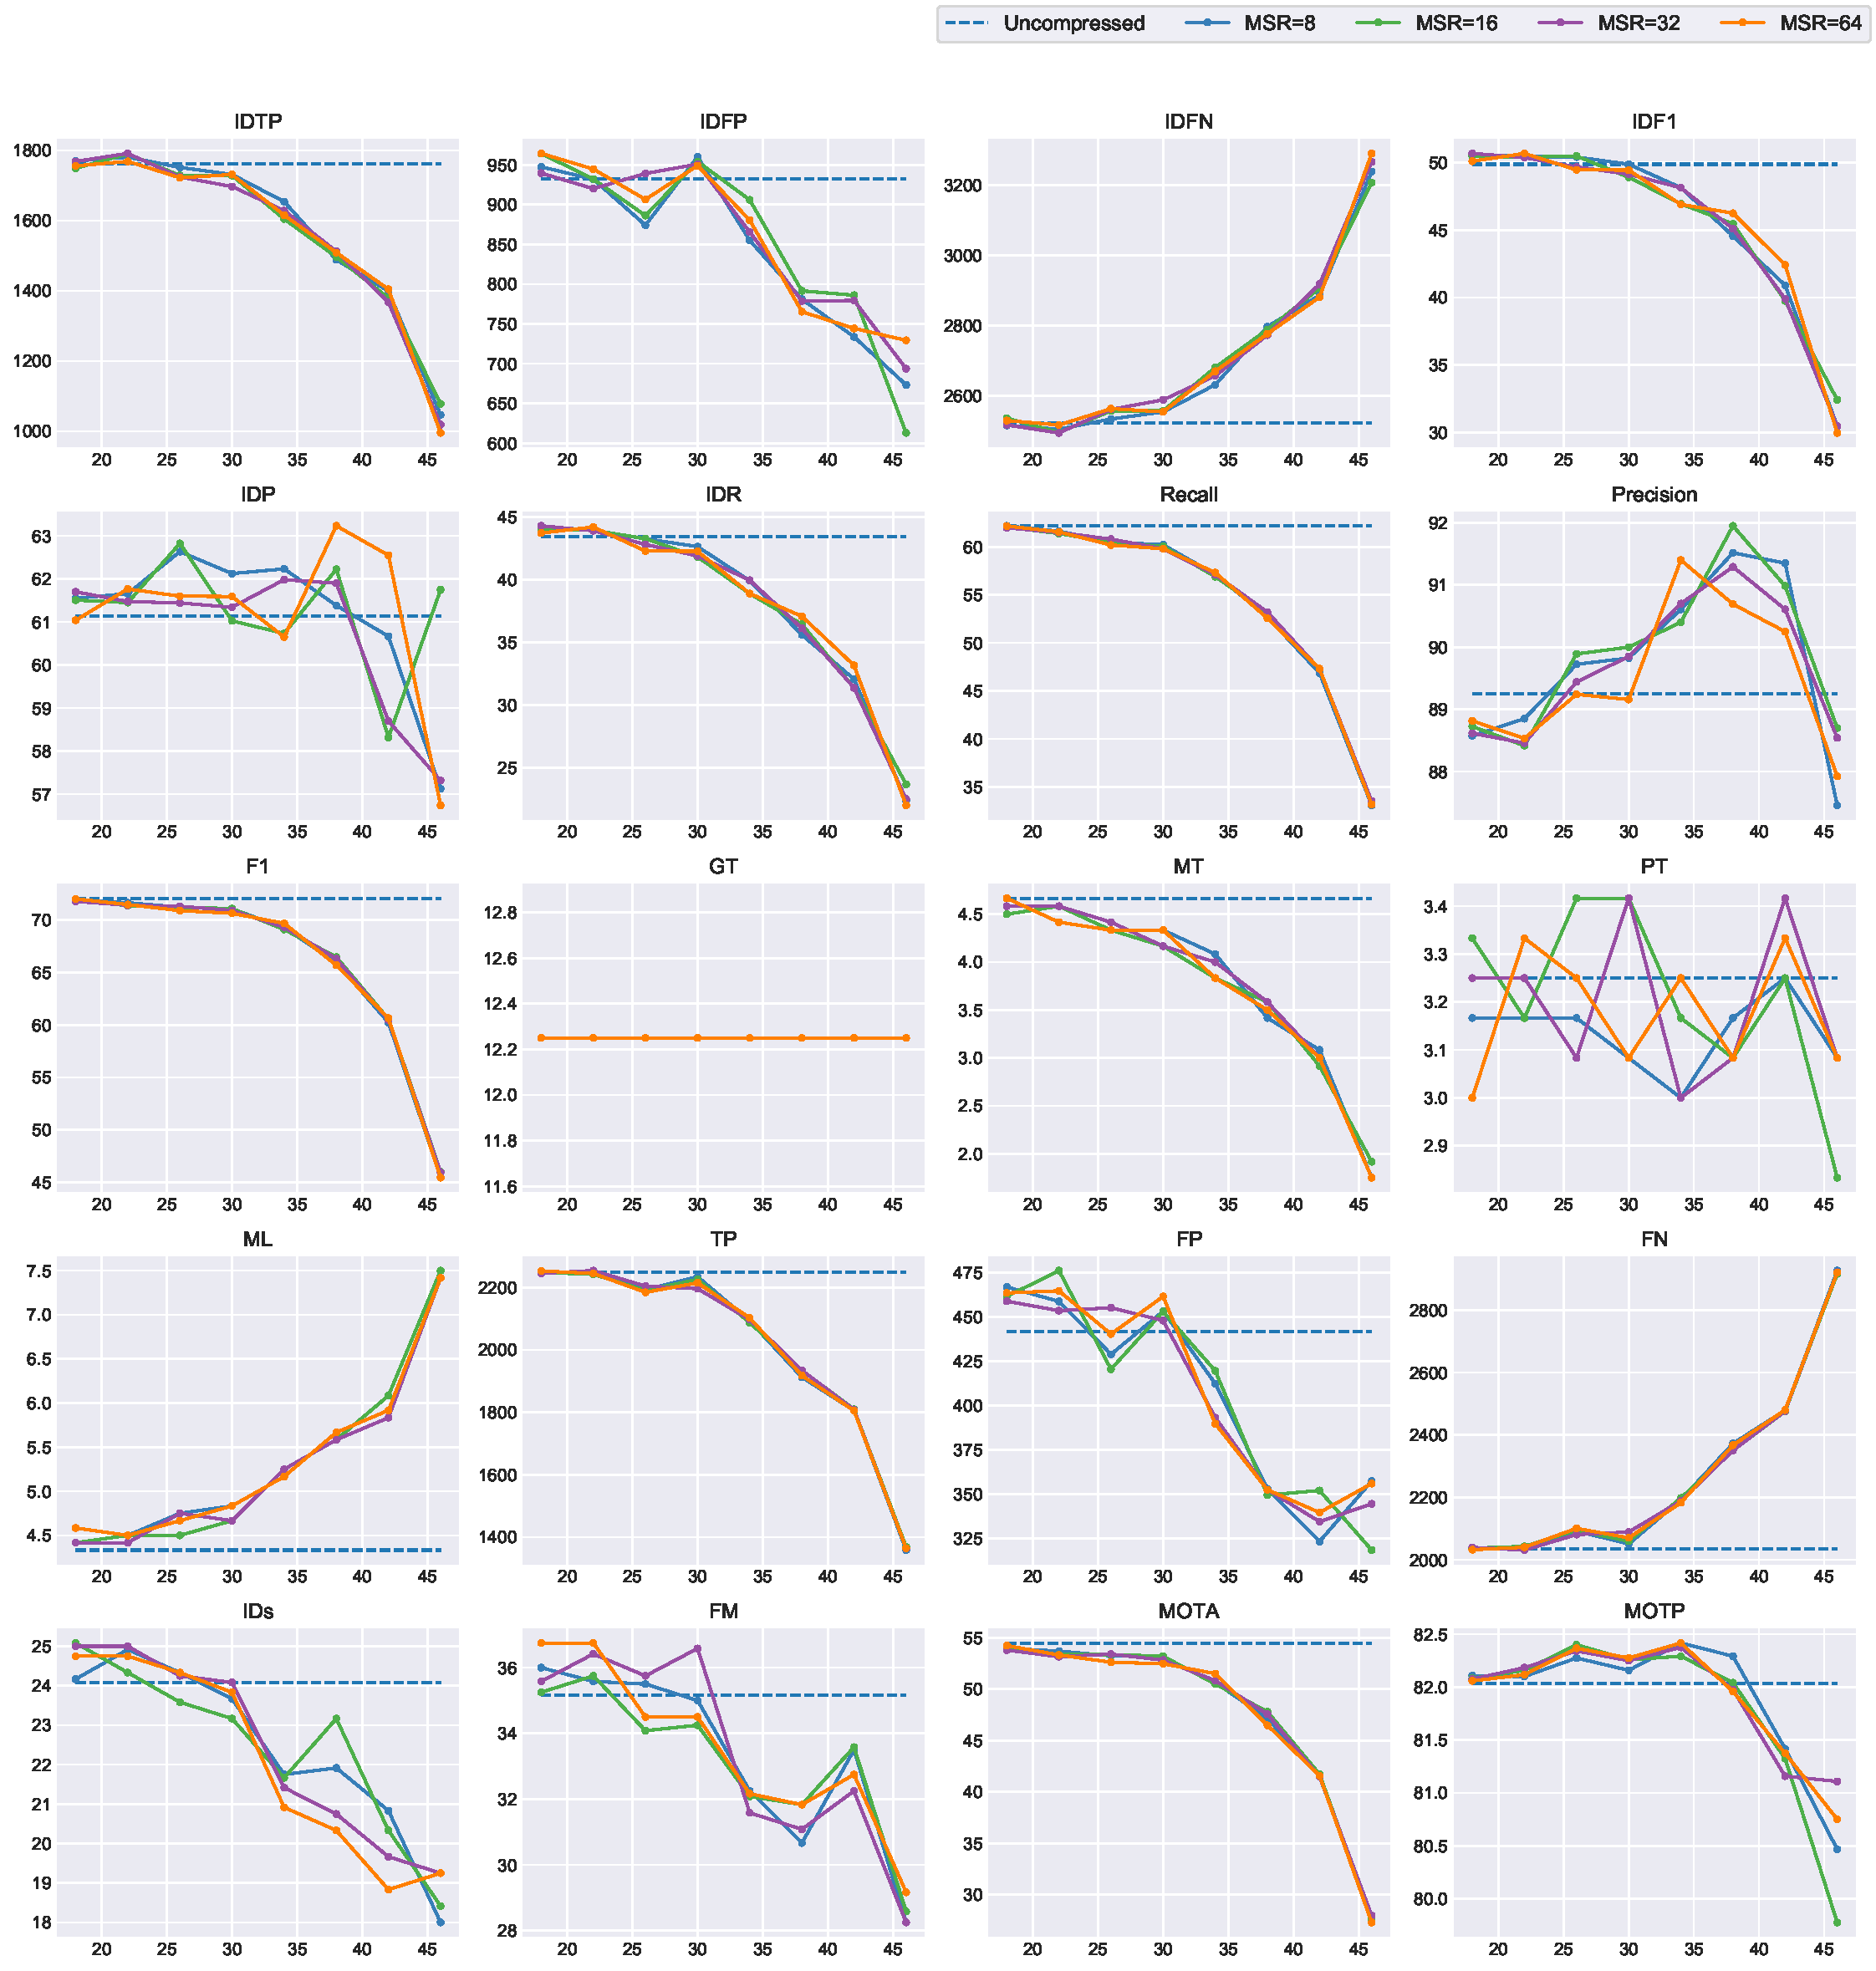
\includegraphics[width=1.0\linewidth]{img/averaged_all_multiplots_qp.pdf}
  \caption[Averaged Result of All Video Samples with All Object Classes]{
    
  }
  \label{fig:averaged_result_all_multiplots_qp}
\end{figure}
\begin{table}[!htbp]
  \centering
  \caption[Averaged performance results of all video samples]
  {Averaged performance results of all video samples.}

  % table for uncompressed
  \begin{subtable}[t]{\linewidth}
    \centering
    \vspace{0pt}
    \resizebox{1.0\linewidth}{!}{
    \begin{tabular}{llrrrrrrrrrrrrrrrrrrrr}
    \toprule
              QP &          MSR &    IDTP &   IDFP &    IDFN &  IDF1 &   IDP &   IDR &  Recall &  Precision &    F1 &    GT &   MT &   PT &   ML &      TP &     FP &      FN &   IDs &    FM &  MOTA &  MOTP \\
    \midrule
    Uncompressed & Uncompressed & 1762.58 & 932.83 & 2522.67 & 49.88 & 61.13 & 43.48 &   62.17 &      89.25 & 72.08 & 12.25 & 4.67 & 3.25 & 4.33 & 2249.75 & 441.67 & 2035.50 & 24.08 & 35.17 & 54.49 & 82.03 \\
    \bottomrule
    \end{tabular}}
    \caption{Mean values for the uncompressed sequence}
  \end{subtable}
 
 
 
  
  % table for msr=8
  \begin{subtable}[t]{\linewidth}
    \centering
    \resizebox{1.0\linewidth}{!}{
    \begin{tabular}{rrrrrrrrrrrrrrrrrrrrrr}
    \toprule
     QP &  MSR &    IDTP &   IDFP &    IDFN &  IDF1 &   IDP &   IDR &  Recall &  Precision &    F1 &    GT &   MT &   PT &   ML &      TP &     FP &      FN &   IDs &    FM &  MOTA &  MOTP \\
    \midrule
     18 &    8 & 1770.08 & 947.50 & 2515.17 & 50.60 & 61.55 & 44.26 &   62.18 &      88.58 & 71.92 & 12.25 & 4.50 & 3.17 & 4.58 & 2246.75 & 466.83 & 2038.50 & 24.17 & 36.00 & 53.97 & 82.11 \\
     22 &    8 & 1780.83 & 931.92 & 2504.42 & 50.46 & 61.66 & 43.96 &   61.62 &      88.85 & 71.65 & 12.25 & 4.58 & 3.17 & 4.50 & 2250.00 & 458.75 & 2035.25 & 24.92 & 35.58 & 53.70 & 82.10 \\
     26 &    8 & 1751.67 & 874.17 & 2533.58 & 50.41 & 62.63 & 43.28 &   60.49 &      89.73 & 71.22 & 12.25 & 4.33 & 3.17 & 4.75 & 2192.92 & 428.92 & 2092.33 & 24.33 & 35.50 & 53.24 & 82.28 \\
     30 &    8 & 1731.50 & 960.08 & 2553.75 & 49.88 & 62.12 & 42.65 &   60.21 &      89.83 & 71.07 & 12.25 & 4.33 & 3.08 & 4.83 & 2234.42 & 453.17 & 2050.83 & 23.67 & 35.00 & 53.13 & 82.16 \\
     34 &    8 & 1653.92 & 855.08 & 2631.33 & 48.14 & 62.23 & 39.93 &   57.12 &      90.61 & 69.26 & 12.25 & 4.08 & 3.00 & 5.17 & 2092.58 & 412.42 & 2192.67 & 21.75 & 32.25 & 50.64 & 82.42 \\
     38 &    8 & 1488.50 & 781.08 & 2796.75 & 44.56 & 61.38 & 35.62 &   52.70 &      91.52 & 65.97 & 12.25 & 3.42 & 3.17 & 5.67 & 1912.42 & 353.17 & 2372.83 & 21.92 & 30.67 & 47.15 & 82.29 \\
     42 &    8 & 1399.25 & 733.83 & 2886.00 & 40.92 & 60.67 & 32.08 &   46.86 &      91.35 & 60.24 & 12.25 & 3.08 & 3.25 & 5.92 & 1805.67 & 323.42 & 2479.58 & 20.83 & 33.50 & 41.48 & 81.42 \\
     46 &    8 & 1046.50 & 673.33 & 3238.75 & 30.48 & 57.12 & 22.40 &   33.09 &      87.46 & 45.48 & 12.25 & 1.75 & 3.08 & 7.42 & 1358.33 & 357.50 & 2926.92 & 18.00 & 28.25 & 27.64 & 80.47 \\
    \bottomrule
    \end{tabular}}
    \caption{Mean values for MSR = 8}
  \end{subtable}
 
 
  
  % table for msr=16
  \begin{subtable}[t]{\linewidth}
    \centering
    \resizebox{1.0\linewidth}{!}{
    \begin{tabular}{rrrrrrrrrrrrrrrrrrrrrr}
    \toprule
     QP &  MSR &    IDTP &   IDFP &    IDFN &  IDF1 &   IDP &   IDR &  Recall &  Precision &    F1 &    GT &   MT &   PT &   ML &      TP &     FP &      FN &   IDs &    FM &  MOTA &  MOTP \\
    \midrule
     18 &   16 & 1749.25 & 964.25 & 2536.00 & 50.48 & 61.51 & 44.07 &   62.04 &      88.73 & 71.88 & 12.25 & 4.50 & 3.33 & 4.42 & 2248.00 & 461.50 & 2037.25 & 25.08 & 35.25 & 54.03 & 82.08 \\
     22 &   16 & 1790.08 & 932.17 & 2495.17 & 50.40 & 61.45 & 43.96 &   61.39 &      88.42 & 71.38 & 12.25 & 4.58 & 3.17 & 4.50 & 2242.17 & 476.08 & 2043.08 & 24.33 & 35.75 & 53.36 & 82.16 \\
     26 &   16 & 1728.75 & 886.25 & 2556.50 & 50.48 & 62.82 & 43.28 &   60.43 &      89.89 & 71.21 & 12.25 & 4.33 & 3.42 & 4.50 & 2190.50 & 420.50 & 2094.75 & 23.58 & 34.08 & 53.36 & 82.40 \\
     30 &   16 & 1728.33 & 954.08 & 2556.92 & 48.91 & 61.02 & 41.83 &   60.04 &      90.00 & 71.10 & 12.25 & 4.17 & 3.42 & 4.67 & 2225.42 & 453.00 & 2059.83 & 23.17 & 34.25 & 53.21 & 82.26 \\
     34 &   16 & 1604.67 & 906.00 & 2680.58 & 46.94 & 60.73 & 38.90 &   56.89 &      90.40 & 69.10 & 12.25 & 3.83 & 3.17 & 5.25 & 2087.08 & 419.58 & 2198.17 & 21.67 & 32.08 & 50.49 & 82.29 \\
     38 &   16 & 1496.58 & 791.58 & 2788.67 & 45.47 & 62.23 & 36.46 &   53.13 &      91.95 & 66.47 & 12.25 & 3.58 & 3.08 & 5.58 & 1934.58 & 349.58 & 2350.67 & 23.17 & 31.83 & 47.81 & 82.04 \\
     42 &   16 & 1379.33 & 786.17 & 2905.92 & 39.76 & 58.32 & 31.38 &   47.28 &      90.98 & 60.56 & 12.25 & 2.92 & 3.25 & 6.08 & 1809.33 & 352.17 & 2475.92 & 20.33 & 33.58 & 41.72 & 81.33 \\
     46 &   16 & 1078.17 & 613.00 & 3207.08 & 32.42 & 61.75 & 23.68 &   33.48 &      88.70 & 45.99 & 12.25 & 1.92 & 2.83 & 7.50 & 1368.58 & 318.58 & 2916.67 & 18.42 & 28.58 & 27.67 & 79.77 \\
    \bottomrule
    \end{tabular}}
    \caption{Mean values for MSR = 16}
  \end{subtable}
 
 
 
  % table for msr=32
  \begin{subtable}[t]{\linewidth}
    \centering
    \resizebox{1.0\linewidth}{!}{
    \begin{tabular}{rrrrrrrrrrrrrrrrrrrrrr}
    \toprule
     QP &  MSR &    IDTP &   IDFP &    IDFN &  IDF1 &   IDP &   IDR &  Recall &  Precision &    F1 &    GT &   MT &   PT &   ML &      TP &     FP &      FN &   IDs &    FM &  MOTA &  MOTP \\
    \midrule
     18 &   32 & 1768.58 & 939.58 & 2516.67 & 50.67 & 61.70 & 44.31 &   61.98 &      88.62 & 71.78 & 12.25 & 4.58 & 3.25 & 4.42 & 2245.33 & 458.83 & 2039.92 & 25.00 & 35.58 & 53.80 & 82.08 \\
     22 &   32 & 1791.42 & 920.08 & 2493.83 & 50.38 & 61.48 & 43.92 &   61.49 &      88.46 & 71.42 & 12.25 & 4.58 & 3.25 & 4.42 & 2254.00 & 453.50 & 2031.25 & 25.00 & 36.42 & 53.15 & 82.18 \\
     26 &   32 & 1724.42 & 939.08 & 2560.83 & 49.68 & 61.44 & 42.82 &   60.80 &      89.44 & 71.32 & 12.25 & 4.42 & 3.08 & 4.75 & 2204.33 & 455.17 & 2080.92 & 24.25 & 35.75 & 53.41 & 82.34 \\
     30 &   32 & 1697.08 & 950.92 & 2588.17 & 49.14 & 61.34 & 41.91 &   59.79 &      89.85 & 70.91 & 12.25 & 4.17 & 3.42 & 4.67 & 2196.08 & 447.92 & 2089.17 & 24.08 & 36.58 & 52.83 & 82.25 \\
     34 &   32 & 1628.42 & 865.50 & 2656.83 & 48.13 & 61.98 & 39.98 &   57.10 &      90.70 & 69.32 & 12.25 & 4.00 & 3.00 & 5.25 & 2096.75 & 393.17 & 2188.50 & 21.42 & 31.58 & 50.83 & 82.38 \\
     38 &   32 & 1512.50 & 778.75 & 2772.75 & 45.10 & 61.90 & 36.13 &   53.20 &      91.29 & 66.31 & 12.25 & 3.58 & 3.08 & 5.58 & 1934.67 & 352.58 & 2350.58 & 20.75 & 31.08 & 47.57 & 81.98 \\
     42 &   32 & 1367.25 & 779.58 & 2918.00 & 39.92 & 58.70 & 31.38 &   47.28 &      90.61 & 60.48 & 12.25 & 3.00 & 3.42 & 5.83 & 1808.25 & 334.58 & 2477.00 & 19.67 & 32.25 & 41.48 & 81.16 \\
     46 &   32 & 1018.67 & 693.75 & 3266.58 & 30.47 & 57.32 & 22.52 &   33.53 &      88.54 & 45.93 & 12.25 & 1.75 & 3.08 & 7.42 & 1363.75 & 344.67 & 2921.50 & 19.25 & 28.25 & 27.97 & 81.11 \\
    \bottomrule
    \end{tabular}}
    \caption{Mean values for MSR = 32}
  \end{subtable}
  
  
  % table for msr=64
  \begin{subtable}[t]{\linewidth}
    \centering
    \resizebox{1.0\linewidth}{!}{
    \begin{tabular}{rrrrrrrrrrrrrrrrrrrrrr}
    \toprule
     QP &  MSR &    IDTP &   IDFP &    IDFN &  IDF1 &   IDP &   IDR &  Recall &  Precision &    F1 &    GT &   MT &   PT &   ML &      TP &     FP &      FN &   IDs &    FM &  MOTA &  MOTP \\
    \midrule
     18 &   64 & 1756.00 & 964.33 & 2529.25 & 50.10 & 61.04 & 43.73 &   62.17 &      88.82 & 72.02 & 12.25 & 4.67 & 3.00 & 4.58 & 2252.83 & 463.50 & 2032.42 & 24.75 & 36.75 & 54.24 & 82.06 \\
     22 &   64 & 1768.75 & 944.75 & 2516.50 & 50.68 & 61.77 & 44.22 &   61.56 &      88.53 & 71.48 & 12.25 & 4.42 & 3.33 & 4.50 & 2244.83 & 464.67 & 2040.42 & 24.75 & 36.75 & 53.33 & 82.12 \\
     26 &   64 & 1722.25 & 906.50 & 2563.00 & 49.46 & 61.60 & 42.30 &   60.18 &      89.24 & 70.90 & 12.25 & 4.33 & 3.25 & 4.67 & 2184.42 & 440.33 & 2100.83 & 24.33 & 34.50 & 52.62 & 82.37 \\
     30 &   64 & 1731.25 & 949.00 & 2554.00 & 49.44 & 61.59 & 42.27 &   59.80 &      89.16 & 70.64 & 12.25 & 4.33 & 3.08 & 4.83 & 2214.75 & 461.50 & 2070.50 & 23.83 & 34.50 & 52.47 & 82.28 \\
     34 &   64 & 1615.58 & 880.42 & 2669.67 & 46.90 & 60.65 & 38.91 &   57.32 &      91.40 & 69.69 & 12.25 & 3.83 & 3.25 & 5.17 & 2102.25 & 389.75 & 2183.00 & 20.92 & 32.17 & 51.51 & 82.42 \\
     38 &   64 & 1508.92 & 765.42 & 2776.33 & 46.25 & 63.23 & 37.09 &   52.56 &      90.69 & 65.69 & 12.25 & 3.50 & 3.08 & 5.67 & 1917.75 & 352.58 & 2367.50 & 20.33 & 31.83 & 46.48 & 81.96 \\
     42 &   64 & 1404.50 & 744.42 & 2880.75 & 42.43 & 62.55 & 33.18 &   47.31 &      90.25 & 60.65 & 12.25 & 3.00 & 3.33 & 5.92 & 1805.17 & 339.75 & 2480.08 & 18.83 & 32.75 & 41.57 & 81.38 \\
     46 &   64 &  995.00 & 729.42 & 3290.25 & 29.98 & 56.74 & 22.02 &   33.18 &      87.92 & 45.43 & 12.25 & 1.75 & 3.08 & 7.42 & 1364.33 & 356.08 & 2920.92 & 19.25 & 29.17 & 27.29 & 80.75 \\
    \bottomrule
    \end{tabular}}
    \caption{Mean values for MSR = 64}
  \end{subtable}

  
\label{tab:averaged_result_all}  
\end{table}
According to the hypothesis stated in Chapter \ref{sec:background/section_e}, the higher the QP, the lower the bitrate and pixel rate, so we expected the tracking performance to be lower. Our performance results from most metrics are consistent with the hypothesis. To describe the decrease of MOTA defined in terms of FP, FN, and IDs based on the equation \ref{eqn:MOTA}, we can see that as QP increases, FP and IDs decreases but FN increases which are consistent with the hypothesis. Although the decrease of FP and IDs contribute to the increase of MOTA, the increase of FN is significantly larger than FP and IDs; thus, we confirmed that MOTA decreases. However, we observed that Precision and MOTP are not consistent with the hypothesis such that the performance increases before the high QP and decreases thereafter. Since each video sample differs in resolution, frame rate, number of objects, and object classes, tracking performance is different. Due to the lack of video samples, the standard deviation is high among the 12 video samples. As there is no insight we can deduce from the standard deviations, we show its table in Appendix \ref{sec:appendix/section_b}. As another visual representation to see if MSR impacts the performance scores, we visualized each performance score on a different MSR as a horizontal axis, and we observed no significant differences on MSR as shown in Figure \ref{fig:averaged_result_all_multiplots_msr}.
\begin{figure}[!htbp]
  \centering
  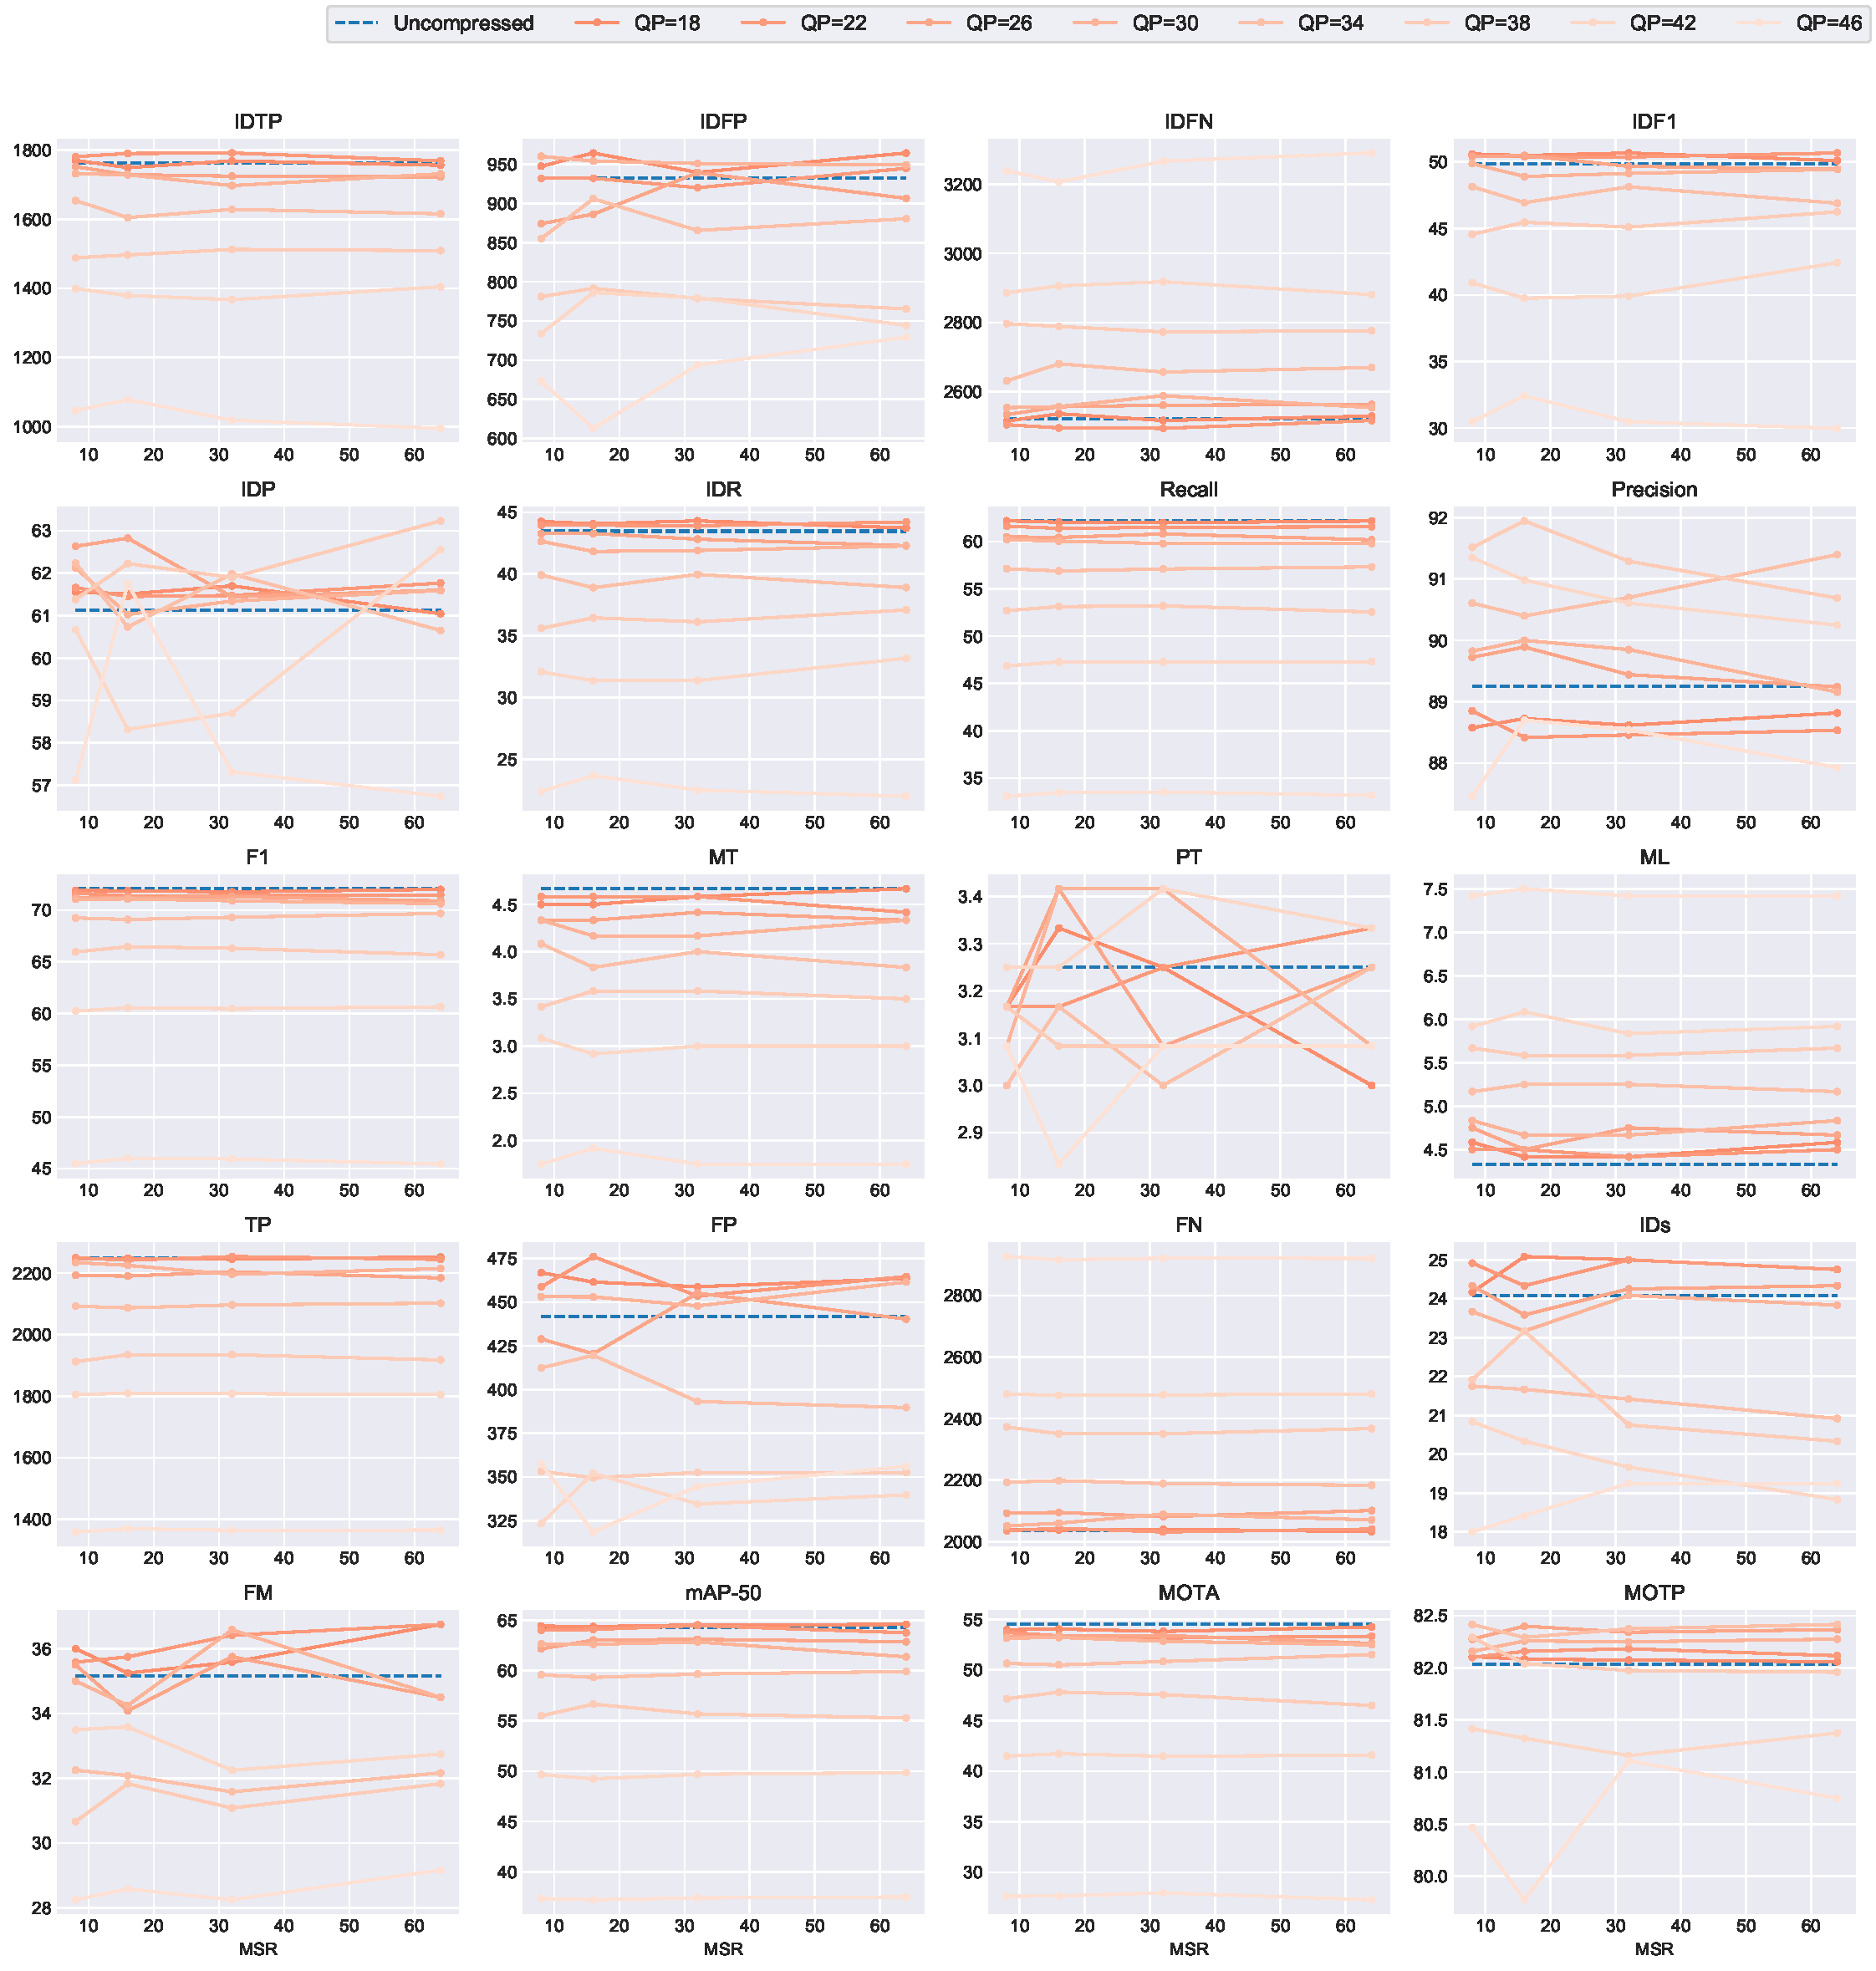
\includegraphics[width=1.0\linewidth]{img/averaged_all_multiplots_msr.pdf}
  \caption[Visualization of the averaged performance results at different MSR of all video samples]
  {Visualization of the average performance results at different MSR across all video samples.}
  \label{fig:averaged_result_all_multiplots_msr}
\end{figure}
To prove the significant impact of QP and MSR on each metric score quantitatively, we conducted a linear regression analysis. Since we have 2 continuous independent variables of QP and MSR on each of the continuous dependent variables of performance metrics score, we applied multiple linear regression on the data shown in Table \ref{tab:averaged_result_all}. We represent the regression model as,
\begin{equation}
Score = \mathit{c_0} + \mathit{c_1} \cdot QP + \mathit{c_2} \cdot MSR + \mathit{c_3} \cdot QP \cdot MSR,
\end{equation}
where $\mathit{c_0}$ is the intercept; $\mathit{c_1}$ and $\mathit{c_2}$ are the coefficients of independent variables QP and MSR; $\mathit{c_3}$ is the coefficient of the interaction term of QP and MSR. Score is each of the performance value from the different metrics. The error term is neglected. Note that we included the interaction term to see if MSR or QP depends on each other. Table \ref{tab:regression} shows the result from the multiple linear regression analysis.
\begin{table}[!htbp]
    \centering
    \caption[Multiple linear regression analysis of averaged performance results]
    {Multiple linear regression analysis of averaged performance results.}
    \resizebox{1.0\linewidth}{!}{
\begin{tabular}{lrrrrrrrrrrrrrrrrrrr}
\toprule
{} &    IDTP &    IDFP &    IDFN &  IDF1 &   IDP &   IDR &  Recall &  Precision &    F1 &    MT &    PT &    ML &      TP &     FP &      FN &   IDs &    FM &  MOTA &  MOTP \\
\midrule
coefficient(Intercept) & 2312.69 & 1169.61 & 1972.56 & 65.29 & 64.37 & 60.56 &   82.86 &      88.28 & 90.22 &  6.55 &  3.41 &  2.30 & 2901.74 & 576.56 & 1383.51 & 29.18 & 40.46 & 72.71 & 83.54 \\
coefficient(QP)        &  -23.05 &  -10.07 &   23.05 & -0.62 & -0.10 & -0.71 &   -0.89 &       0.05 & -0.76 & -0.09 & -0.01 &  0.09 &  -27.78 &  -5.34 &   27.78 & -0.21 & -0.23 & -0.78 & -0.05 \\
coefficient(MSR)       &    0.10 &   -0.23 &   -0.10 & -0.02 & -0.01 & -0.02 &   -0.00 &       0.00 & -0.00 &  0.00 & -0.00 &  0.00 &   -0.06 &  -0.07 &    0.06 &  0.02 &  0.02 & -0.00 & -0.01 \\
coefficient(QP*MSR)    &   -0.01 &    0.01 &    0.01 &  0.00 &  0.00 &  0.00 &    0.00 &      -0.00 & -0.00 & -0.00 &  0.00 & -0.00 &    0.00 &   0.00 &   -0.00 & -0.00 & -0.00 & -0.00 &  0.00 \\
p-value(Intercept)     &    0.00 &    0.00 &    0.00 &  0.00 &  0.00 &  0.00 &    0.00 &       0.00 &  0.00 &  0.00 &  0.00 &  0.00 &    0.00 &   0.00 &    0.00 &  0.00 &  0.00 &  0.00 &  0.00 \\
p-value(QP)            &    0.00 &    0.00 &    0.00 &  0.00 &  0.05 &  0.00 &    0.00 &       0.21 &  0.00 &  0.00 &  0.13 &  0.00 &    0.00 &   0.00 &    0.00 &  0.00 &  0.00 &  0.00 &  0.00 \\
p-value(MSR)           &    0.98 &    0.87 &    0.98 &  0.88 &  0.74 &  0.88 &    0.98 &       0.93 &  0.99 &  0.89 &  0.42 &  0.89 &    0.99 &   0.91 &    0.99 &  0.54 &  0.62 &  1.00 &  0.73 \\
p-value(QP*MSR)        &    0.92 &    0.73 &    0.92 &  0.88 &  0.76 &  0.88 &    0.98 &       0.79 &  1.00 &  0.87 &  0.36 &  0.88 &    0.99 &   0.87 &    0.99 &  0.37 &  0.70 &  0.98 &  0.66 \\
\bottomrule
\end{tabular}
    }
    \label{tab:regression}
\end{table}
To see if the independent variable is statistically significant on the dependent variable, we conducted a hypothesis test at a significance level of 0.05. The null hypothesis is the case the coefficient is 0 ($H_0: c_i = 0$) and the alternative hypothesis is the case the coefficient is not zero ($H_1: c_i \neq 0$). From the table, the p-value of QP is less than or equal to 0.05 except Precision and PT, while all of the p-values of MSR and the interaction term of $QP \cdot MSR$ is greater than 0.05. This shows that we reject the null hypothesis on QP, so QP significantly impacts most metrics at 95\% confidence. However, we fail to reject the null hypothesis for MSR and the interaction term of QP and MSR. Hence, it is insufficient to prove that MSR and the interaction term are statistically significant on each metric. We estimated that MSR does not impact the object tracking performance, and QP and MSR do not depend on each other; therefore, our hypothesis for MSR, as explained in Chapter \ref{sec:background/section_e}, is inconsistent with our results. Thus, we will limit our study to QP only.

We just showed the averaged result from the multiple video sequences, but we will justify further by analyzing the individual sequences.

